%!TEX root = ../main.tex
% !TeX encoding = UTF-8
\section{Wearables como Sistemas Processados} \label{chap:revisao_bibliografica}

   Aqui será descrito os principais conceitos do trabalho, além de suas tecnologias e metodologias. Ao final será descritos pesquisas relacionadas.

   \subsection{Fundamentação do Conceito Wearable}
      % Introdução histórica e geral
      Sistemas \wearables\ são sistemas que, com a possibilidade de ter um computador acoplado ao corpo, proporciona ao usuário um nível superior de informações contextualizadas dentro de um ambiente interativo \cite{Amorim2017}.

      %Com a tecnologia constantemente melhorando à medida que a informação se torna sem-fio, os avanços demandaram mais fatores móveis e \wearable\ de produtos que possuem acesso à informação.
      %Segundo \cite{Gemperle1998}, um produto que é \wearable, deveria ter sua `\textit{wearability}' sendo este definido como a interação entre o corpo humano e o objeto \textit{wearable} estendendo ao corpo em movimento.

      Devido ao movimento de seus usuários, um controlador \wearable\ é embutido em um ambiente \mobile\ e necessita-se da interação com o ambiente ao seu redor.
      Com a distribuição espacial dos módulos pelo corpo, a comunicação torna-se um item importante em termos consumo de energia e com isso,
      %A rede de comunicação é uma mistura de conexões cabeadas e sem-fios.
      a comunicação sem-fio é a tecnologia predominante por causa da necessidade de mobilidade e gasto consciente \cite{Plessl2003, Kymissis1998}.



      %wearable precisa ser pequeno
      A introdução desses no ambiente de científico não é nova como é reportado por \cite{Sutherland1968, Mann1996, Mann1997}.
      Entretanto, a aplicação desses dispositivos, depende diretamente da miniaturização dos componentes eletrônicos.
      %aparicão nos dias atuais
      %Esse fenômeno fica claro ao perceber o crescente espaço ganho pelos \textit{smartwatches}, \textit{fitness trackers}, óculos, equipamentos de realidade virtual e aumentada e muitos outros equipamentos embarcados nas atividades pessoais de usuários.
      %Com esses novos dispositivos embarcados de propósito geral miniaturizados, aumenta-se a sua atração devido à fácil disponibilidade dos dispositivos, baixo preço e ferramentas de desenvolvimento disponíveis para desenvolvimento de aplicações específicas incluindo compiladores e sistemas operacionais para tal, mas não são otimizados para uso \wearable.
      %Segundo \cite{Plessl2003}, muitos dos sistemas \wearables\ construídos possuíam características diferentes de componentes que prestam auxílio à tarefas pessoais de usuários com base no paradigma de operações \textit{hands-free} e a propriedade de computação \wearable\ discreta.
      %Sistemas de computação distribuídos no corpo construídos a partir desses equipamentos interativos são altamente ineficientes devido à falta de especialização de componentes individuais de propósito específico.

      Segundo \cite{Hennessy2011}, por mais que exista um leque de processadores para sistemas embutidos, o preço é um dos fatores mais importantes para seu \design, sendo tão importante quanto o requisito de desempenho pois, necessita-se de um desempenho elevado a um preço reduzido.

      Esses dispositivos embarcados podem também trabalhar de forma colaborativa com \textit{smartphones}, redes e outros sistemas criando um sistema mais complexo \cite{Jozwiak2017}.

      A utilização de \hardware\ reconfigurável nos permite alcançar alto poder de processamento com eficiência energética em relação à processadores para tarefas de computação intensiva em tempo real, por exemplo \cite{Plessl2003}.


   \subsection{\textit{Field-Programmable Logic Device} (FPGA)}
      % uso de fpga no mundo
      %Até recentemente, os \hardwares\ reconfiguráveis eram utilizados unicamente na protitipação de projetos de circuitos integrados de aplicação especifica (ASIC, do inglês \textit{application-specific integrated circuit} e produção em baixo volume por causa de sua baixa velocidade e custo por unidade.
      %Entretanto, com a variedade desses dispositivos disponibilizados hoje no mercado, em conjunto com a elevação do custo de engenharia não recorrente (NRE, do inglês \textit{Nonrecurring Engineering}, que refere-se ao custo de pesquisa, \design, desenvolvimento e teste de um novo produto e exigências de mercado), houve um crescente interesse na utilização de FPGAs para sistemas embutidos devido suas vantagens sobre ASICs em termos de flexibilidade de projeto e custo zero de engenharia não recorrente citada \cite{Mei2000}.
      %lousa branca
      %Tais dispositivos, juntos com sua plataforma de interação, de forma geral, permitem ao \designer\ de sistemas embutidos ter uma \textit{lousa branca} em que possa implementar \hardwares\ computacionais personalizados tão facilmente como o desenvolvimento de um \software, como foi possível ilustrar na Figura \ref{fig:rt-board}.

      % Plataforma FPGA
      Uma \textit{plataforma FPGA} é um chip na qual, além de conter o componente FPGA, está integrado à inúmeras interfaces e componentes e seus respectivos circuitos.
      Como possui recursos suficientes para a sintetização de circuitos complexos, é possível implementar inúmeros projetos digitais como funções de processamento de imagem, algoritmos de redes de computadores, criptográficos e \textit{soft}-processadores completos, cada projeto de acordo com os recursos disponíveis \cite{Plessl2003}.
      %Entretanto, enquanto configurar um \hardware\ reconfigurável é uma tarefa fácil graças às ferramentas disponíveis hoje, criar um \design\ de \hardware\ inicial não é \cite{Sass2010}.

      %\begin{figure}[h] \centering
      %   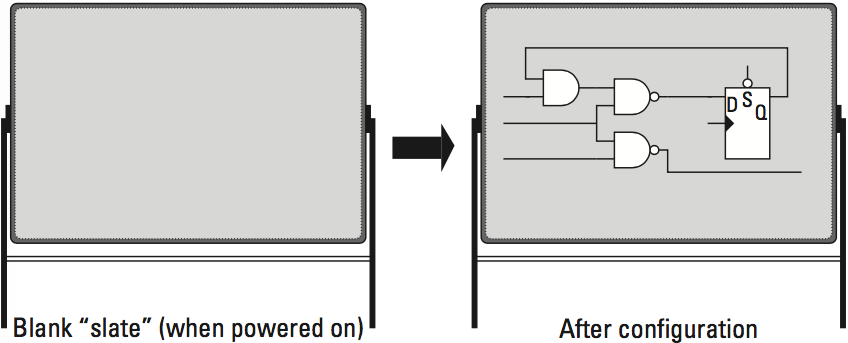
\includegraphics[width=0.75\textwidth]{img/rt-board.png}
      %   \caption{Ilustração em alto nível do funcionamento interno do FPGA. Fonte: \cite{Sass2010}.}
      %   \label{fig:rt-board}
      %\end{figure}

      %A seguir, será descrito a tecnologia que consiste os \hardwares\ reconfiguráveis, em especial o FPGA, e as respectivas linguagens de descrição de \hardware.

   %\subsection{Sua Tecnologia}
      % PLD
      %Para introduzir alguns conceitos, é importante destacar o que são os dispositivos lógicos programáveis (PLDs, do inglês \textit{Programable Logic Devices}).
      %Às vezes chamados de dispositivos lógico programáveis em campo (FPLD, do inglês \textit{Field-Programmable Logic Device}), podem ser adaptados para criar muitos dispositivos digitais, desde simples portas lógicas até estruturas complexas.
      %\cite{tocci2003sistemas, Plessl2003} dizem que com um investimento de capital pequeno, qualquer empresa pode comprar os \softwares\ de desenvolvimento e \hardware\ necessário para programar PLDs para seus projetos digitais.
      %De modo geral, os PLDs são descritos como pertencendo a três tipo diferentes sendo eles os dispositivos lógicos programáveis simples (SPLD), dispositivos lógicos programáveis complexos (CPLDs, do inglês \textit{Complex Programmable Logic Devices}) e arranjo de portas programáveis em campo (FPGA) sendo o último tipo abordado neste trabalho \cite{Brown1996}.

      %LUTS
      O FPGA segundo \cite{tocci2003sistemas}, constitui-se de vários módulos lógicos programáveis, relativamente pequenos, independentes e interconectados, para criar funções maiores.
      %Cada módulo lida, normalmente, com até quatro ou cinco variáveis de entrada.
      %A maioria dos FPGAs utilizam uma \textit{look-up table} (LUT) para criar as funções lógicas desejadas.
      %Uma LUT funciona como uma tabela-verdade, no sentido que a saída é programada para criar a função combinacional armazenando valores verdadeiros e falsos adequado a cada combinação de entrada.
      Os recursos de roteamento de sinal programável dentro do chip tendem a ser bem variados, com extensões de caminhos diferentes disponíveis, adequando a cada sintetização.
      %Os atrasos de sinal em um projeto dependem do roteamento real de sinal selecionado pelo \software\ de programação.
      %Os módulos lógicos também contêm registradores programáveis.
      Eles não são associados a nenhum pino de entrada e saída (I/O, do inglês \textit{Input and Output}).
      Em vez disso, cada pino de I/O é conectado ao bloco programável de entrada e saída que, por sua vez, é conectado aos módulos lógicos com linhas de roteamento selecionadas.

      %\begin{figure}[!t] \centering
      %   \vspace{-10pt}
      %   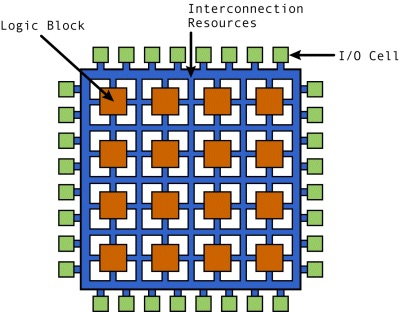
\includegraphics[width=0.5\textwidth]{img/rt-arch_fpga.jpg}
      %   \vspace{-15pt}
      %   \caption{Exemplo da arquitetura internas de um FPGA. Fonte: \url{http://www.eetimes.com/document.asp?doc_id=1274496}. Acesso: 30/05/2017.}
      %   \label{fig:rb-arch_fpga}
      %\end{figure}

      %Uma arquitetura geral simplista de FPGA é exibido na Figura~\ref{fig:rb-arch_fpga}.
      %Nela os quadrados menores situado nas laterais são blocos de I/O que podem ser configurados para fornecer recursos de entrada, saída ou bidirecionais.
      %Os quadrados maiores situados no interior são as LUTs, usados para guardar dados que entram ou saem e realizar as operações lógicas.
      %Os canais que interligam os blocos entre si são estabelecidas por meio de conexões que passam pelas linhas e colunas nos canais entre esses blocos e possuem a funcionalidade de serem interconexões programáveis \cite{tocci2003sistemas}.
      %A tecnologia interna de um FPGA consiste basicamente de um arranjo de blocos lógicos, canais de roteamento para interconexão de blocos lógicos e blocos de entrada e saída de sinais em torno do circuito.
      %FPGAs baseado em SRAM (do inglês \textit{Static Random Access Memory}) utilizam células SRAM para controlar a funcionalidade de blocos lógicos e entrada e saída de sinais bem como as rotas, e pode ser reprogramado arbitrariamente em nível de circuito, muitas vezes, baixando um novo \textit{stream} de dados de configuração para o dispositivo.
      Esses dispositivos possuem milhões de portas de lógicas programáveis, bilhões de transistores, além de outros blocos de \hardware\ dedicados como memórias embarcadas e multiplicadores de ponto-fixo tornando-os um dos circuitos integrados (CI) mais densos existente \cite{Choi2016}.

      % tecnologia e energia
      Segundo \cite{tocci2003sistemas},
      %tais maravilhas de flexibilidade de projetos digital podem fornecer uma série de opções de projeto sendo voltados para indústria e até mesmo educação.
      ao utilizar tecnologia CMOS, o consumo de energia do chip é relativamente baixo comparado com outras tecnologias podendo ser confeccionado em nível de tensão elétrica, frequências e cargas para os sinais de I/O.
      %O mercado fornece diferentes graus de velocidade de FPGA a fim de que o projetista utilize o mais adequado ao projeto.
      %Entretanto, um dispositivo FPGA pode ser configurado para um número infinito de projetos e isso implica na não possibilidade de afirmar o montante de dissipação de energia para um dispositivo FPGA.
      %O \software\ Quartus II tem duas ferramentas para estimular o montante de uso de energia para uma aplicação.
      %O \textit{PowerPlay Early Power Estimator} é usado durante os estágios iniciais do projeto para estimar a magnitude de potência do dispositivo.
      Dessa forma, FPGAs são chips que podem ser programados instantaneamente para funções de qualquer circuito digital \cite{Choi2016}.

      % Importancia
      %\cite{tocci2003sistemas, Plessl2003} citam ainda que o motivo de PLDs estarem dominando o mercado é o fato de que, como são dispositivos programáveis, a mesma funcionalidade pode ser obtida com um circuito integrado (CI) ao invés de diversos circuitos individuais.
      Isso significa maior confiabilidade, menor espaço ocupado na placa, consumo de energia, complexidade de desenvolvimento e, geralmente, menor custo de fabricação.

      \subsubsection{\textit{Hard} e \textit{Software Cores}}
         % Utilização de um processador sintético ou físico
         A unidade de processamento central (CPU, do inglês \textit{Central Processing Unit}) nesses tipos de sistema pode estar disposta em duas naturezas distintas, sendo estas \textit{hard} e \textit{soft} \cores.
         A primeira é um \core\ dedicado, ou seja, um pedaço de circuito integrado dentro (ou não) de um FPGA, enquanto a segunda é feita por meio da sintetização de um processador no FPGA utilizando seus recursos lógicos, ou seja, \design\ e sintetização na placa.
         Independente de sua natureza, o sistema, cujo nome torna-se SoC FPGA (do inglês, \textit{System-on-Chip} FPGA), terá a seguinte arquitetura exibida na Figura~\ref{fig:rb-soc}.
         
         \begin{figure}[h] 
            \centering
            \vspace{-1em}
            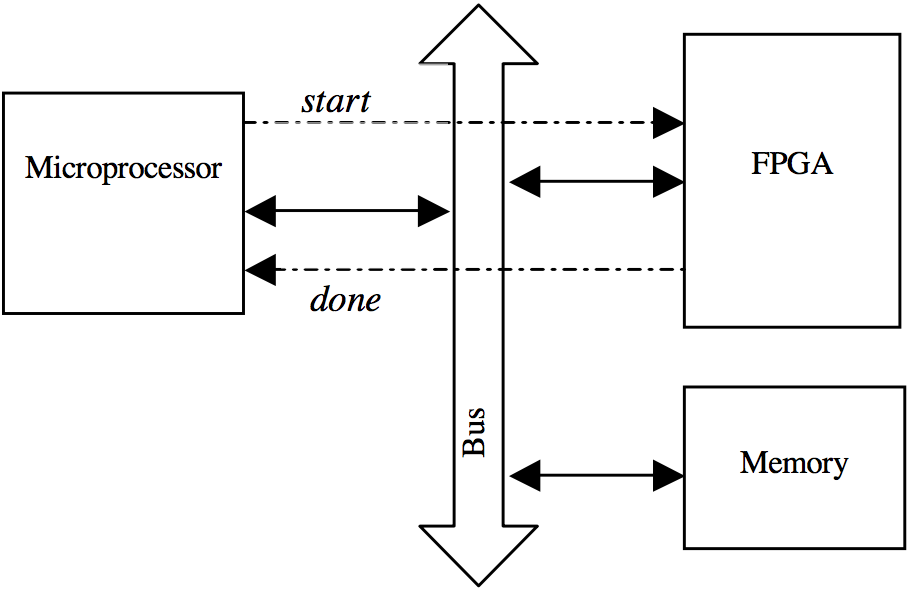
\includegraphics[width=0.35\textwidth]{img/into-soc.png}
            \caption{Visão geral de um SoC FPGA. As setas representam os barramentos de comunicação entre os principais componentes.}
            \label{fig:rb-soc}
         \end{figure}
         
         Cada um tipo de \core\ possui suas vantagens.
         Ao utilizar um \textit{hard} \core, é possível utilizar todos seus recursos obtendo máxima performance nas atividades executadas, a utilização de um \textit{soft} \core\ permite a extensão/configuração de sua arquitetura \cite{Plessl2003}.

         %Um das maiores barreiras para o \design\ de projetos em FPGA é a necessidade de uso de linguagens de descrição de \hardware.
         %Elas serão descritas a seguir.

   \subsection{Profiling} \label{sec:profile}
         \Profile\ é uma procedimento para auxiliar o desenvolvedor a coletar informações do \software\ em tempo de execução.

         O processo é feito ao colocar o \software\ referencial (programa a ser analisado) como entrada representativa na ferramenta e a coleta é realizada em várias partes da aplicação ao longo de sua execução neste.
         Uma das técnicas do \profile\ de mensurar uma aplicação é na realização de interrupções periódica no programa e amostrar o seu \textit{program counter}.
         Dessa forma, é possível utilizar um histograma para contar quando um programa é interrompido em um endereço particular e a partir dessa informação, calcular a fração aproximada do tempo total de execução gasto em suas partes \cite{Graham1982}.
         %Distribuições GNU/Linux possuem a ferramenta \texttt{gprof} na qual avalia procedimentos enviados por parâmetro, realizando o cálculo de tais informações de \software\ \cite{Graham1982}.
